% Provenance (never printed): see sources/outline_sources.md (Year 3: Gibbs
% energy and the phase rule in rocks, chemical potential recalled from the
% chemistry book; ternary diagrams; pseudosections, principle). Brief:
% sources/book5/BRIEFS.md, ch. 11. Curves from figdata/bachelor-3/
% gasp_tables.py, schreinemakers.py and regular_solution.py. Exercise and
% problem values in the Book 5 scratch calculator calc/ch11.py.
\chapter{Thermodynamics of Rocks}\label{ch:b3:petrological-thermodynamics}

A garnet a few millimetres across grew zone by zone as its schist was buried
and heated. Its rim still records, in its calcium, iron and magnesium, the
last equilibrium it reached with the biotite and plagioclase around it. The
Year 2 volume turned such compositions into a temperature and a pressure with
two calibrated equations. This chapter opens the box: where the equations
come from, how far tables of measured enthalpies and entropies can be
trusted, how many minerals a rock can hold, how solid solutions mix and
unmix, and how a computer turns a bulk composition into a map of the
assemblages it should show.

\begin{recall}
The Gibbs energy, the chemical potential, the activity and the equilibrium
constant, the variance and the phase rule, the miscibility gap and the lever
rule are in the chemistry books' university volumes. The univariant reaction,
its Clapeyron slope $\Delta_rS/\Delta_rV$, the invariant point and the
aluminosilicate diagram computed from tables are in the Year 2 volume, in its
chapter on metamorphic facies; the geothermometer and geobarometer, the
garnet--biotite exchange thermometer and the GASP barometer, in its chapter on
P--T--t paths; ternary diagrams and the cotectic, in its chapter on magmas. A
solid solution and its end members are in the Year 1 volume, in its chapter on
minerals.
\end{recall}

\section{Equilibrium from tables}\label{sec:b3:petrological-thermodynamics:tables}

For a reaction among minerals of fixed composition, equilibrium at the
temperature $T$ and pressure $P$ is $\Delta_rG(T, P) = 0$. Tables give, at
\qty{298.15}{K} and \qty{1}{bar}, the enthalpy of formation, the entropy and
the molar volume of each mineral, and the heat capacity $C_p(T)$ above. The
Year 2 volume took $\Delta_rH$, $\Delta_rS$ and $\Delta_rV$ as constants. The
general result is the following.

\begin{theorem}[Gibbs energy of a reaction at $T$ and $P$]\label{thm:b3:petrological-thermodynamics:dg}
Let a reaction have, at $T_0 = \qty{298.15}{K}$ and \qty{1}{bar}, the
enthalpy $\Delta_rH^\circ$ and entropy $\Delta_rS^\circ$, the heat capacity
change $\Delta_rC_p(T)$ and, among solids, a volume change $\Delta_rV$
independent of $T$ and $P$. Then
\[
  \Delta_rG(T, P) = \Delta_rH^\circ + \int_{T_0}^{T}\Delta_rC_p\,\mathrm dT
  - T\Bigl(\Delta_rS^\circ + \int_{T_0}^{T}\frac{\Delta_rC_p}{T}\,\mathrm dT\Bigr)
  + (P - 1)\,\Delta_rV ,
\]
and the equilibrium line is $P = 1 - \Delta_rG(T, 1)/\Delta_rV$.
\end{theorem}

\begin{proof}
At \qty{1}{bar}, $(\partial\Delta_rH/\partial T)_P = \Delta_rC_p$ and
$(\partial\Delta_rS/\partial T)_P = \Delta_rC_p/T$; integrating from $T_0$
gives $\Delta_rH(T)$ and $\Delta_rS(T)$, and $\Delta_rG = \Delta_rH -
T\Delta_rS$. At fixed $T$, $(\partial\Delta_rG/\partial P)_T = \Delta_rV$,
constant by hypothesis; integrating from 1 to $P$ adds $(P - 1)\Delta_rV$.
Setting $\Delta_rG(T, P) = 0$ gives the line.
\end{proof}

The two integrals partly cancel: their sum is $\int_{T_0}^T\Delta_rC_p(1 -
T/T')\,\mathrm dT'$, in which the factor $1 - T/T'$ is negative and small
where $T'$ is close to $T$. Among solids, $\Delta_rC_p$ is itself small,
because the heat capacity of a mineral is nearly the sum of those of its
oxides. The constant-property approximation is therefore good, and the
tables say how good. For the GASP reaction,
\[
  \ce{3 CaAl2Si2O8 <=> Ca3Al2Si3O12 + 2 Al2SiO5 + SiO2},
\]
the summary table gives $\Delta_rH^\circ = \qty{-36.3}{kJ}$,
$\Delta_rS^\circ = \qty{-130.7}{J.K^{-1}}$ and $\Delta_rV =
\qty{-6.61}{J.bar^{-1}}$, so a line of slope \qty{19.8}{bar/K}; the
high-temperature tables, which include the heat capacities, give
$\Delta_rG$ at each \qty{100}{K}, and the two lines differ by less than
\qty{0.12}{kbar} up to \qty{1200}{K} (the figure below).
% ledger: rh95:gasp-298, rh95:gasp-ht

The experiments do not agree as well. Reversed in a piston-cylinder press at
900 to \qty{1250}{\celsius}, the reaction lies \qty{0.9}{kbar} higher than the
tables at \qty{627}{\celsius} and \qty{1.9}{kbar} higher at
\qty{927}{\celsius}. With $\Delta_rV = \qty{-6.61}{J.bar^{-1}}$,
\qty{1.9}{kbar} is an error of \qty{12.6}{kJ} in $\Delta_rH$; the
uncertainties of the four enthalpies of formation, \qty{3.2}{kJ} for
grossular, \qty{2.0}{kJ} for anorthite and kyanite, \qty{1.0}{kJ} for
quartz, combine to about \qty{8}{kJ} in $\Delta_rH$. Calorimetry fixes each
mineral to a few kilojoules; a reaction among large formula units multiplies
these errors and divides them by a small volume change.
% ledger: rh95:gasp-298, kn88:gasp

\begin{definition}[Internally consistent thermodynamic dataset]\label{def:b3:petrological-thermodynamics:dataset}
An \emph{internally consistent thermodynamic dataset}\index{internally
consistent thermodynamic dataset} is a table of the standard properties of
many minerals and fluids (enthalpy of formation, entropy, volume, heat
capacity, thermal expansion and compressibility) adjusted together, within the
uncertainties of calorimetry, so that every equilibrium computed from it
passes through the reversed experiments on which it was fitted.
\end{definition}

Such a dataset is fitted once, by weighted least squares or by linear
programming over all the brackets at once, and then used for every
reaction among its minerals, including reactions never studied in the
laboratory. Its numbers are not independent measurements: one enthalpy may
be shifted by a kilojoule to fit a reaction it takes part in. Values from
different datasets must never be mixed.

\begin{omfigure}
\begin{tikzpicture}
\begin{axis}[omrecord, width=0.78\linewidth, height=0.5\linewidth,
  xlabel={temperature (\unit{\celsius})}, ylabel={pressure (\unit{kbar})},
  xmin=400, xmax=1300, ymin=0, ymax=30, legend style={font=\scriptsize,
  at={(0.03,0.97)}, anchor=north west, legend cell align=left}]
% computed in figdata/bachelor-3/gasp_tables.py
\fill[omLithLime!60] (axis cs:900,19) rectangle (axis cs:1250,28);
\addplot[red!70!black, very thick] table[x=tc, y=p_kn88] {figdata/out/bachelor-3-gasp_tables-lines.dat};
\addlegendentry{experiment (end members)}
\addplot[omDef, thick, densely dashed] table[x=tc, y=p_const] {figdata/out/bachelor-3-gasp_tables-lines.dat};
\addlegendentry{tables, constant $\Delta_rH$, $\Delta_rS$}
\addplot[omDef, only marks, mark=*, mark size=1.8pt] table[x=tc, y=p_table] {figdata/out/bachelor-3-gasp_tables-tables.dat};
\addlegendentry{tables, with heat capacities}
\node[font=\scriptsize, align=center] at (axis cs:1075,26.3) {reversed\\experiments};
\node[font=\scriptsize] at (axis cs:560,4) {anorthite};
\node[font=\scriptsize, align=center] at (axis cs:560,17) {grossular + kyanite\\+ quartz};
\end{axis}
\end{tikzpicture}

\par\smallskip{\small The end-member GASP reaction, 3 anorthite = grossular +
2 kyanite + quartz, computed from the calorimetric tables with constant
properties (dashed) and with the heat capacities (dots), and the line fitted
to reversed experiments made in the shaded range (red, extrapolated below
\qty{900}{\celsius}).}\label{fig:b3:petrological-thermodynamics:gasp}
\end{omfigure}
% ledger: rh95:gasp-298, rh95:gasp-ht, kn88:gasp

\section{The phase rule in rocks}\label{sec:b3:petrological-thermodynamics:phase-rule}

The phase rule of chemistry gives the variance $F = c - p + 2$ of a system of
$c$ components in $p$ phases. A rock is such a system, and its minerals show
which part of the pressure--temperature plane it equilibrated in.

\begin{proposition}[Mineralogical phase rule]\label{prop:b3:petrological-thermodynamics:goldschmidt}
A rock that has reached equilibrium at a pressure and temperature chosen
freely within an area of the pressure--temperature plane holds at most as
many phases as it has components: $p \le c$. This is the
\emph{mineralogical phase rule}\index{mineralogical phase rule}.
\end{proposition}

\begin{proof}
The phase rule gives $F = c - p + 2$ independent intensive variables. If the
pressure and temperature can both vary without changing the assemblage, two
of them are free: $F \ge 2$, so $p \le c$. A rock with $p = c + 1$ phases lies
on a univariant line; with $p = c + 2$, at an invariant point; neither is
likely for a rock picked at random.
\end{proof}

A rock that breaks the rule either equilibrated on a reaction line, which its
textures may show, or never reached equilibrium as a whole: corona textures,
zoned minerals and relict grains are common reasons. Counting components
needs care. A component held only in one phase of fixed composition, such as
zircon, can be dropped with its phase; a component fixed by an external
reservoir, such as water when a fluid flows through the rock, is not counted
as free, since its chemical potential is imposed.

Around an invariant point, the univariant lines do not cross at random. In a
system of $c$ components, $c + 2$ phases meet at the point and $c + 2$
reactions radiate from it, each written among $c + 1$ phases and named after
the phase it omits, in brackets.

\begin{definition}[Schreinemakers analysis]\label{def:b3:petrological-thermodynamics:schreinemakers}
\emph{Schreinemakers analysis}\index{Schreinemakers analysis} is the method
that arranges the univariant lines around an invariant point from the
compositions of the phases alone, before any measurement of their
thermodynamic properties: it fixes the order of the lines, the side of each
line that is stable, and the assemblages of each sector between them.
\end{definition}

\begin{method}[Schreinemakers' rules]\label{met:b3:petrological-thermodynamics:schreinemakers}
(1) Write the $c + 2$ reactions, each without one phase. (2) Each line is
stable on one side of the point and metastable on the other. (3) The
metastable extension of the ($i$) line, which omits the phase $i$, lies in a
sector where $i$ is stable. (4) No sector between two consecutive stable lines
spans more than \ang{180}. (5) Across a line, the assemblages on either side
are those of the two sides of its reaction. Fixing one line with data then
fixes the whole bundle, up to a mirror image.
\end{method}

The aluminosilicate triple point of the Year 2 volume is the simplest case,
$c = 1$ and three lines. The figure below shows a two-component case
computed by minimising the Gibbs energy at every point.

\begin{omfigure}
\begin{tikzpicture}
\begin{axis}[omrecord, width=0.62\linewidth, height=0.5\linewidth,
  xlabel={temperature (\unit{\celsius})}, ylabel={pressure (\unit{kbar})},
  xmin=400, xmax=800, ymin=1, ymax=9, grid=none]
% computed in figdata/bachelor-3/schreinemakers.py
\addplot[omDef, very thick] table[x=t, y=p] {figdata/out/bachelor-3-schreinemakers-ray_A_s.dat};
\addplot[omDef, thick, densely dashed] table[x=t, y=p] {figdata/out/bachelor-3-schreinemakers-ray_A_m.dat};
\addplot[omDef, very thick] table[x=t, y=p] {figdata/out/bachelor-3-schreinemakers-ray_B_s.dat};
\addplot[omDef, thick, densely dashed] table[x=t, y=p] {figdata/out/bachelor-3-schreinemakers-ray_B_m.dat};
\addplot[omDef, very thick] table[x=t, y=p] {figdata/out/bachelor-3-schreinemakers-ray_C_s.dat};
\addplot[omDef, thick, densely dashed] table[x=t, y=p] {figdata/out/bachelor-3-schreinemakers-ray_C_m.dat};
\addplot[omDef, very thick] table[x=t, y=p] {figdata/out/bachelor-3-schreinemakers-ray_D_s.dat};
\addplot[omDef, thick, densely dashed] table[x=t, y=p] {figdata/out/bachelor-3-schreinemakers-ray_D_m.dat};
\node[font=\scriptsize, fill=white, inner sep=1pt] at (axis cs:740,7.85) {(A)};
\node[font=\scriptsize, fill=white, inner sep=1pt] at (axis cs:540,8.75) {(C)};
\node[font=\scriptsize, fill=white, inner sep=1pt] at (axis cs:540,1.6) {(B)};
\node[font=\scriptsize, fill=white, inner sep=1pt] at (axis cs:740,2.15) {(D)};
\node[font=\scriptsize, align=center] at (axis cs:592,7.7) {A + B\\B + D};
\node[font=\scriptsize, align=center] at (axis cs:450,5.0) {A + D};
\node[font=\scriptsize, align=center] at (axis cs:592,2.4) {A + C\\C + D};
\node[font=\scriptsize, align=center] at (axis cs:765,5.0) {A + B\\B + C\\C + D};
\end{axis}
\end{tikzpicture}

\par\smallskip{\small A Schreinemakers bundle in a two-component system with
four phases of compositions A (0), B ($1/3$), C ($2/3$) and D (1),
computed for invented properties: stable lines solid, metastable extensions
dashed, and the stable pairs in each sector. (D) is A + C = 2B, (A) is B + D =
2C, (C) is 2A + D = 3B and (B) is A + 2D = 3C.}\label{fig:b3:petrological-thermodynamics:schreinemakers}
\end{omfigure}

\section{Solid solutions}\label{sec:b3:petrological-thermodynamics:solutions}

Most rock-forming minerals are solid solutions, and their end members appear
in reactions through their activities. The Year 2 volume took $a = X^3$ for
the grossular in a garnet and $a = X$ for the anorthite in a plagioclase.
Both are cases of one model.

\begin{definition}[Site-mixing activity model]\label{def:b3:petrological-thermodynamics:site-mixing}
In a \emph{site-mixing activity model}\index{site-mixing activity model}, the
ions of a mineral mix at random on each crystallographic site, independently
of the other sites. The ideal activity of an end member is then the product,
over the sites, of the fraction of each site it fills raised to the number of
such sites per formula unit: $a_i = \prod_s X_{s,i}^{\,n_s}$.
\end{definition}

A garnet $X_3Y_2\ce{Si3O12}$ has three dodecahedral sites $X$ for
\ce{Ca}, \ce{Fe}, \ce{Mg} and \ce{Mn}: $a_{\text{grossular}} =
X_{\text{Ca}}^3$. A garnet with $X_{\text{Ca}} = 0.10$ holds
\qty{10}{\percent} of grossular, but its activity is $10^{-3}$. The ideal
model counts the configurations; real solutions also have an excess energy,
because ions of different sizes strain the lattice.

\begin{definition}[Gibbs energy--composition diagram]\label{def:b3:petrological-thermodynamics:gx}
A \emph{Gibbs energy--composition diagram}\index{Gibbs energy--composition
diagram} plots, at fixed temperature and pressure, the molar Gibbs energy of
each phase of a system against its composition. The stable assemblage of any
bulk composition lies on the lower convex hull of the curves: a single phase
where its curve is on the hull, two phases at the ends of a common tangent.
\end{definition}

\begin{proposition}[Regular solution]\label{prop:b3:petrological-thermodynamics:regular}
In a binary solution with one mixing site per formula unit and the
interaction energy $W$, the Gibbs energy of mixing is
\[
  G_{\text{mix}} = RT\bigl[x\ln x + (1 - x)\ln(1 - x)\bigr] + Wx(1 - x).
\]
If $W > 0$, the solution is stable at every composition above $T_c =
W/(2R)$; below $T_c$ the curve has two inflections and the compositions
between the two points of its common tangent split into two phases.
\end{proposition}

\begin{proof}
The first term is $-T$ times the configurational entropy of random mixing;
the second, the simplest excess energy, symmetric and zero at both ends.
Differentiating twice, $G''_{\text{mix}} = RT/[x(1 - x)] - 2W$. Its minimum
over $x$ is at $x = 1/2$, where it equals $4RT - 2W$, which is positive for
every $x$ if $T > W/(2R)$. Below, $G''_{\text{mix}} < 0$ on an interval
around $1/2$: the curve bends down there, a straight line between two points
of the curve lies below it, and by the definition above the rock is two
phases.
\end{proof}

\begin{definition}[Solvus, exsolution]\label{def:b3:petrological-thermodynamics:solvus}
The \emph{solvus}\index{solvus} is the curve, in the temperature--composition
plane, that bounds the miscibility gap of a solid solution: below it, a
single crystal of intermediate composition is unstable and splits into two.
\emph{Exsolution (mineral)}\index{exsolution (mineral)} is that splitting
within a crystal on cooling: lamellae of one composition grow in a host of the
other.
\end{definition}

Alkali feldspars, pyroxenes and amphiboles show exsolution lamellae,
visible under the microscope or to the eye: the perthite of many granites is
an exsolved alkali feldspar, a potassium-rich host with sodium-rich
lamellae. Between the \omterm{def:b3:petrological-thermodynamics:solvus}{solvus} and the spinodal, where $G''_{\text{mix}} = 0$,
a crystal must first nucleate the second phase; inside the spinodal, any small
fluctuation of composition grows by diffusion alone.

\begin{omfigure}
\begin{tikzpicture}
\begin{groupplot}[group style={group size=2 by 1, horizontal sep=1.7cm},
  omrecord, width=0.47\linewidth, height=0.42\linewidth, title style={font=\small},
  legend style={font=\scriptsize, legend cell align=left}]
\nextgroupplot[title={(a) Gibbs energy of mixing}, xlabel={$x$},
  ylabel={$G_{\text{mix}}$ (\unit{kJ.mol^{-1}})}, xmin=0, xmax=1, ymin=-9, ymax=1,
  legend style={at={(0.5,0.03)}, anchor=south}]
% computed in figdata/bachelor-3/regular_solution.py
\addplot[black, thick, densely dotted] table[x=x, y=g1500] {figdata/out/bachelor-3-regular_solution-gx.dat};
\addlegendentry{\qty{1500}{K}}
\addplot[red!70!black, thick, densely dashed] table[x=x, y=g1203] {figdata/out/bachelor-3-regular_solution-gx.dat};
\addlegendentry{$T_c = \qty{1203}{K}$}
\addplot[omDef, thick] table[x=x, y=g0900] {figdata/out/bachelor-3-regular_solution-gx.dat};
\addlegendentry{\qty{900}{K}}
\addplot[omDef, thin, forget plot] coordinates {(0.111,-0.635) (0.889,-0.635)};
\nextgroupplot[title={(b) solvus and a section at $X_0 = 0.3$}, xlabel={$x$},
  ylabel={temperature (\unit{K})}, xmin=0, xmax=1, ymin=600, ymax=1300,
  legend style={at={(0.5,0.03)}, anchor=south}]
\addplot[omDef, thick] table[x=x, y=t_bin] {figdata/out/bachelor-3-regular_solution-solvus.dat};
\addlegendentry{solvus}
\addplot[black, thick, densely dotted] table[x=x, y=t_spin] {figdata/out/bachelor-3-regular_solution-solvus.dat};
\addlegendentry{spinodal}
\addplot[red!70!black, thick, forget plot] coordinates {(0.3,600) (0.3,1300)};
\addplot[red!70!black, thick, densely dashed] table[x=x2, y=t] {figdata/out/bachelor-3-regular_solution-section.dat};
\addlegendentry{isopleths at $X_0$}
\addplot[red!70!black, thick, densely dashed, forget plot] table[x=x1, y=t] {figdata/out/bachelor-3-regular_solution-section.dat};
\node[font=\scriptsize] at (axis cs:0.5,1250) {one phase};
\node[font=\scriptsize] at (axis cs:0.5,950) {two phases};
\end{groupplot}
\end{tikzpicture}

\par\smallskip{\small A regular solution with $W = \qty{20}{kJ.mol^{-1}}$
(illustrative). (a) Gibbs energy of mixing at three temperatures; at
\qty{900}{K} the common tangent (thin line) touches the curve at $x = 0.11$
and 0.89. (b) The \omterm{def:b3:petrological-thermodynamics:solvus}{solvus} and the spinodal; a rock of bulk composition $X_0 =
0.3$ (vertical red line) is one phase above \qty{1136}{K} and two phases
below, whose compositions follow the \omterm{def:b3:petrological-thermodynamics:solvus}{solvus} (dashed).}\label{fig:b3:petrological-thermodynamics:solvus}
\end{omfigure}

\section{Pseudosections}\label{sec:b3:petrological-thermodynamics:pseudosections}

Panel (b) of the figure above is already a small \omterm{def:b3:petrological-thermodynamics:pseudosection}{pseudosection}: for one bulk
composition, it says which phases are stable at each temperature, and what
their compositions and proportions are. A metamorphic rock has some ten
components and many solid solutions, but the principle is the same.

\begin{definition}[Gibbs energy minimisation]\label{def:b3:petrological-thermodynamics:minimisation}
\emph{Gibbs energy minimisation}\index{Gibbs energy minimisation} finds, at a
given temperature and pressure, the set of phases, their compositions and
their amounts that minimises the total Gibbs energy of a system of fixed bulk
composition, subject to the conservation of each component.
\end{definition}

\begin{definition}[Pseudosection, isopleth, effective bulk composition]\label{def:b3:petrological-thermodynamics:pseudosection}
A \emph{pseudosection}\index{pseudosection} is a phase diagram, usually in
the pressure--temperature plane, computed for one fixed bulk composition: it
is divided into fields, each labelled by the assemblage that minimises the
Gibbs energy there. An \emph{isopleth (pseudosection)}\index{isopleth
(pseudosection)} is a line of a pseudosection along which a compositional
variable of one phase, or its amount, is constant. The \emph{effective bulk
composition}\index{effective bulk composition} is the part of the rock's
composition that still takes part in the equilibrium, once the cores of zoned
crystals, porphyroblasts sealed off from the matrix and other isolated
material are removed.
\end{definition}

A \omterm{def:b3:petrological-thermodynamics:pseudosection}{pseudosection} does not show univariant lines in the sense of the Year 2
volume: in a system with solid solutions, the boundary between two fields is
where one phase appears or disappears, and its position depends on the bulk
composition. Reading one is direct. The observed assemblage fixes a field;
the measured composition of a mineral, the calcium of a garnet rim for
instance, picks an isopleth inside it; a second isopleth, of another element
or another mineral, crosses it at the pressure and temperature of
equilibrium. Zoned garnets carry a sequence of such crossings, one for each
zone, along the path of the rock. But as the garnet grows its core takes
manganese and calcium out of reach of the matrix: the \omterm{def:b3:petrological-thermodynamics:pseudosection}{effective bulk
composition} changes, and the \omterm{def:b3:petrological-thermodynamics:pseudosection}{pseudosection} must be recomputed for the
later zones.

\begin{inthelab}[The petrologist's desk]
\begin{minipage}[t]{0.55\linewidth}\vspace{0pt}
The petrologist first studies a thin section under the polarising
microscope, to identify the assemblage, its textures and which grains grew
together. The same section, coated with carbon, then goes into an electron
microprobe, which measures the composition of spots a few micrometres across
along profiles through the garnets. Software that minimises the Gibbs energy
with an internally consistent dataset and a set of activity models computes
a \omterm{def:b3:petrological-thermodynamics:pseudosection}{pseudosection} for the bulk composition, measured on a slice of the same
rock. The isopleths of the measured compositions are plotted on it, and where
they cross is the answer. The uncertainty of the dataset and of the activity
models, not that of the measurements, usually limits it.
\end{minipage}\hfill
\begin{minipage}[t]{0.42\linewidth}\vspace{0pt}
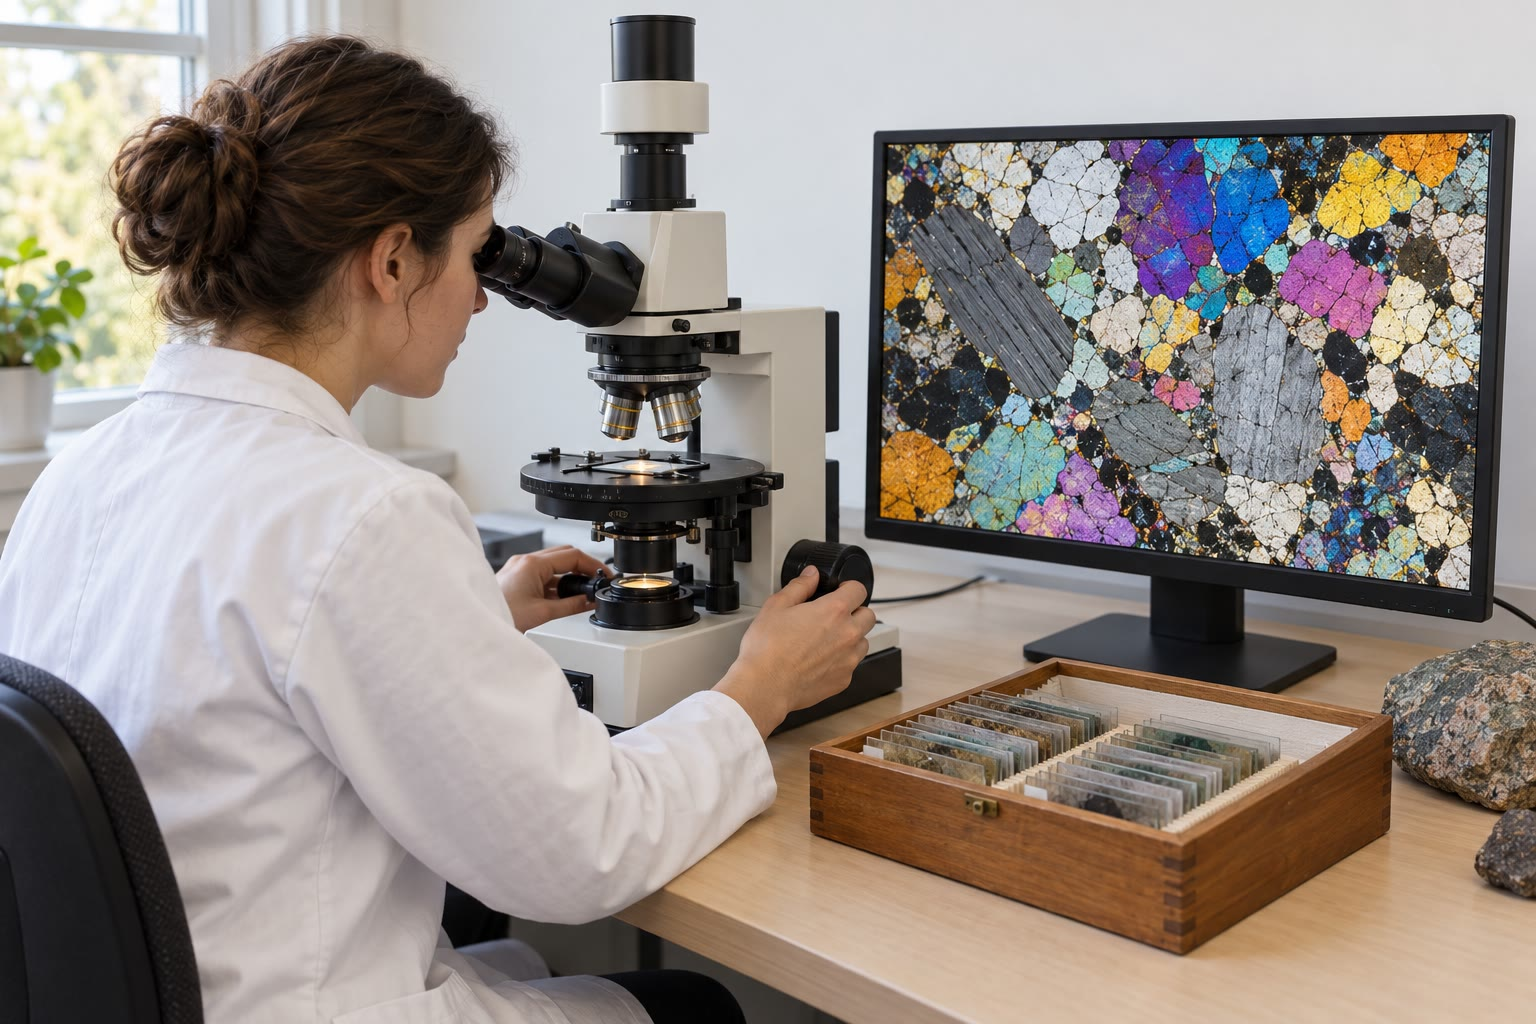
\includegraphics[width=\linewidth]{images/book5/ai/b3-petrology-desk.jpg}

{\scriptsize A petrologist at a polarising microscope, a box of thin
sections at hand and a thin section in polarised light on the screen
(AI-generated illustration).}
\end{minipage}
\end{inthelab}

\section{Exercises}

\begin{exercise}[$\star$]\label{exo:b3:petrological-thermodynamics:1}
From the tables, albite has $\Delta_fH^\circ = \qty{-3935.0}{kJ}$, $S^\circ =
\qty{207.4}{J.K^{-1}}$, $V = \qty{100.07}{cm^3}$; jadeite $-3029.3$, 133.5,
60.40; quartz $-910.7$, 41.5, 22.69 (per mole). For albite = jadeite + quartz,
compute $\Delta_rH$, $\Delta_rS$, $\Delta_rV$ (in \unit{J.bar^{-1}}), the
Clapeyron slope and the pressure of the line at \qty{600}{\celsius} with
constant properties.
\end{exercise}
% ledger: rh95:ab-jd-qz

\begin{exercise}[$\star$]\label{exo:b3:petrological-thermodynamics:2}
A rock of the system \ce{MgO}--\ce{SiO2} holds forsterite, enstatite and
quartz. Apply the \omterm{prop:b3:petrological-thermodynamics:goldschmidt}{mineralogical phase rule}. What do you conclude?
\end{exercise}

\begin{exercise}[$\star$]\label{exo:b3:petrological-thermodynamics:3}
Compute the ideal activities of grossular and pyrope in a garnet with
$X_{\text{Ca}} = 0.20$ and $X_{\text{Mg}} = 0.15$, and of anorthite in a
plagioclase with $X_{\text{an}} = 0.40$ (one site).
\end{exercise}

\begin{exercise}[$\star$]\label{exo:b3:petrological-thermodynamics:4}
Compute the critical temperature of a regular solution with $W =
\qty{15}{kJ.mol^{-1}}$. What $W$ gives $T_c = \qty{1000}{K}$?
\end{exercise}

\begin{exercise}[$\star\star$]\label{exo:b3:petrological-thermodynamics:5}
At \qty{1000}{K}, the tables give the Gibbs energies of formation
$-5432.2$ (grossular), $-3478.1$ (anorthite), $-2088.8$ (kyanite) and $-730.2$
(quartz), in \unit{kJ.mol^{-1}}. Compute $\Delta_rG$ of the GASP reaction at
\qty{1}{bar} and its equilibrium pressure, and compare with the experimental
line $P_0 = 22.80\,T - 1093$ (bar, \unit{\celsius}).
\end{exercise}
% ledger: rh95:gasp-ht, kn88:gasp

\begin{exercise}[$\star\star$]\label{exo:b3:petrological-thermodynamics:6}
For the regular solution of the figure ($W = \qty{20}{kJ.mol^{-1}}$), compute
$G_{\text{mix}}$ at $x = 0.5$ and \qty{900}{K}, then at the \omterm{def:b3:petrological-thermodynamics:solvus}{solvus} limb $x =
0.111$. Show that splitting a crystal of composition 0.5 into the two limbs
lowers its Gibbs energy, and by how much.
\end{exercise}

\begin{exercise}[$\star\star$]\label{exo:b3:petrological-thermodynamics:7}
How many phases meet at an invariant point, and how many univariant lines
radiate from it, in a system of three components? In the bundle of the
figure, check that each of the four reactions is balanced.
\end{exercise}

\begin{exercise}[$\star\star$]\label{exo:b3:petrological-thermodynamics:8}
A rock of bulk composition $X_0 = 0.3$ in the regular solution of the figure
has cooled to \qty{900}{K}, where the \omterm{def:b3:petrological-thermodynamics:solvus}{solvus} limbs are 0.111 and 0.889.
Compute the proportion of each phase.
\end{exercise}

\begin{exercise}[$\star\star$]\label{exo:b3:petrological-thermodynamics:9}
With the GASP barometer $P = P_0 + (3RT/6.21)\ln(X_{\text{Ca}}/X_{\text{an}})$
(bar), compute $\partial P/\partial X_{\text{an}}$ at \qty{900}{K} and
$X_{\text{an}} = 0.30$. By how much does an error of 0.01 in $X_{\text{an}}$
move the pressure?
\end{exercise}

\begin{exercise}[$\star\star\star$]\label{exo:b3:petrological-thermodynamics:10}
Show that the spinodal of a regular solution is $x(1 - x) = RT/(2W)$. At what
temperature does a crystal of composition 0.3 become unstable to any small
fluctuation, for $W = \qty{20}{kJ.mol^{-1}}$? Compare with the temperature at
which it reaches the \omterm{def:b3:petrological-thermodynamics:solvus}{solvus}, $T = W(1 - 2x)/[R\ln((1 - x)/x)]$, and explain
the gap.
\end{exercise}

\begin{exercise}[$\star\star\star$]\label{exo:b3:petrological-thermodynamics:11}
Show that the \omterm{def:b3:petrological-thermodynamics:solvus}{solvus} of a symmetric regular solution satisfies $RT\ln[x/(1 -
x)] + W(1 - 2x) = 0$, and that it reaches its maximum, $T_c = W/(2R)$, at $x
= 1/2$.
\end{exercise}

\begin{exercise}[$\star\star\star$]\label{exo:b3:petrological-thermodynamics:12}
A rock holds \qty{2.0}{wt\percent} \ce{MnO}. Garnet cores containing
\qty{10}{wt\percent} \ce{MnO} make up \qty{8}{wt\percent} of the rock and are
sealed off from the matrix. Compute the \ce{MnO} content of the \omterm{def:b3:petrological-thermodynamics:pseudosection}{effective bulk
composition}. Why does it matter for the \omterm{def:b3:petrological-thermodynamics:pseudosection}{pseudosection} of the garnet rims?
\end{exercise}

\section{Problem: The Garnet of the Varden Schist}

\begin{problem}[{Weekend problem --- the pressure and temperature of an
invented schist, from tables, the phase rule, activity models and
thermobarometry}]
\label{pb:b3:petrological-thermodynamics:1}
% values: calc/ch11.py; gasp_tables.py
The schist of the Varden Hills basement, metamorphosed about
\qty{480}{Ma} ago, holds garnet, biotite, muscovite, plagioclase, kyanite and
quartz. At the rim of a garnet and in the grains around it, the microprobe
gives: garnet $X_{\text{Fe}} = 0.74$, $X_{\text{Mg}} = 0.12$, $X_{\text{Ca}} =
0.10$, $X_{\text{Mn}} = 0.04$; biotite $\ce{Mg}/(\ce{Mg} + \ce{Fe}) = 0.45$;
plagioclase $X_{\text{an}} = 0.30$. Use the tables of this chapter for the
GASP reaction, the Year 2 volume's thermometer
\[
T = \frac{52\,635 + 0.311P}{20.20 - 3R\ln K_D}\quad(T \text{ in K}, P
\text{ in bar}),
\]
and its experimental barometer $P = 22.80\,t - 1093 + (3RT/6.21)\ln
(X_{\text{Ca}}/X_{\text{an}})$, with $t$ in \unit{\celsius} and $T$ in
kelvin. Take $R = \qty{8.314}{J.mol^{-1}.K^{-1}}$, a crustal density of
\qty{2800}{kg/m^3} and $g = \qty{9.81}{m/s^2}$.

\medskip\noindent\textbf{Part I --- The tables.}
\begin{enumerate}
  \item From the summary table, compute $\Delta_rH^\circ$, $\Delta_rS^\circ$
        and $\Delta_rV$ of the GASP reaction.
  \item Compute $\Delta_rG$ at \qty{298.15}{K} and \qty{1}{bar}. Which side
        is stable at the surface?
  \item Compute the end-member pressure at \qty{900}{K} with constant
        properties, and the Clapeyron slope.
  \item The high-temperature tables give $\Delta_rG = \qty{81.5}{kJ}$ at
        \qty{900}{K} and \qty{119.8}{kJ} at \qty{1200}{K} (\qty{1}{bar}).
        Compute the pressures.
  \item Compare with the experimental line at the same temperatures.
  \item What error in $\Delta_rH$ would explain the gap at \qty{1200}{K}?
        Compare with the combined uncertainty of the four enthalpies.
  \item Why do the heat capacities change the result so little?
\end{enumerate}

\medskip\noindent\textbf{Part II --- The phase rule.}
\begin{enumerate}[resume]
  \item List the components needed to describe the six minerals and a water
        fluid, and count the phases.
  \item Compute the variance with the phase rule, and check the \omterm{prop:b3:petrological-thermodynamics:goldschmidt}{mineralogical
        phase rule}.
  \item A second sample holds kyanite and sillimanite side by side. What does
        it say about its pressure and temperature?
  \item Water flowed through the rock during metamorphism. How does that
        change the count?
\end{enumerate}

\medskip\noindent\textbf{Part III --- Activities and thermobarometry.}
\begin{enumerate}[resume]
  \item Compute the ideal activities of grossular and anorthite, and $\ln K$
        of the GASP reaction in the rock.
  \item Compute $K_D$ of the garnet--biotite exchange.
  \item Compute the temperature at \qty{8}{kbar}.
  \item Compute the GASP pressure at that temperature.
  \item Iterate to the intersection of the two equations.
  \item Redo the intersection with the end-member line of the tables in place
        of the experimental line (with $\Delta_rV = \qty{-6.61}{J.bar^{-1}}$).
        Which result do you keep, and why?
  \item By how much does an error of 0.05 in $X_{\text{an}}$ move the
        result?
\end{enumerate}

\medskip\noindent\textbf{Part IV --- The burial.}
\begin{enumerate}[resume]
  \item With the constant properties of the Year 2 volume, kyanite =
        sillimanite has $\Delta_rH = \qty{7.7}{kJ}$, $\Delta_rS =
        \qty{12.6}{J.K^{-1}}$, $\Delta_rV = \qty{0.571}{J.bar^{-1}}$. Is the
        result in the kyanite field?
  \item Compute the depth of burial.
  \item The garnet core has $X_{\text{Ca}} = 0.07$ and grew with plagioclase
        of the same $X_{\text{an}}$, at about the same temperature. Was the
        core formed deeper or shallower than the rim?
  \item Give the peak pressure and depth of burial of the Varden schist.
\end{enumerate}
\end{problem}
